
\documentclass[10pt,a4paper]{article}
\usepackage[utf8]{inputenc}
\usepackage[french]{babel}
\usepackage{amsmath}
\usepackage{graphicx}
\usepackage[left=2cm,right=2cm,top=2cm,bottom=2cm]{geometry}

\author{Jérôme Hue, Damien Carreau}
\title{Traitement du signal - Compte rendu}

\begin{document}
\maketitle
\section{La fonction Transformée de Fourrier Discrète}
\noindent
Données : \\
On échantillone la fonction entre $a$  = -50 secondes et $b$ = 50 secondes, avec un total de $N$ = 32768 échntillons.\\
La période d'échantillonage est : \( T_e = \dfrac{(b-a)}{N} = \dfrac{1}{327,68} \) \\
La fréquence d'échantillonage est : \( f_e = \dfrac{1}{T_e} = 327,68 \) \\
Intervalle de fréquence
L'intervalle entre deux échantillons en fréquence est de fe/N = 1/100.


\begin{figure}[h]
\begin{center}
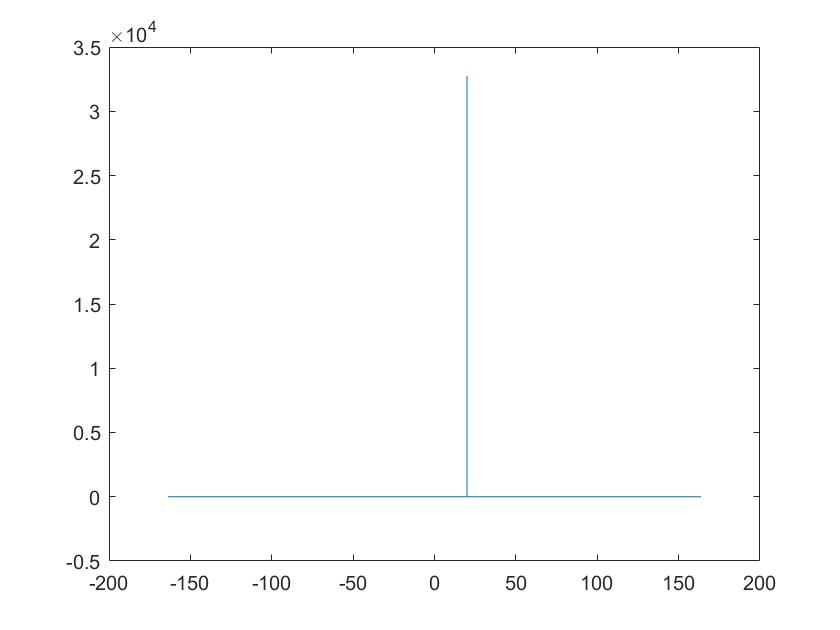
\includegraphics[scale=0.35]{tf_fct3.jpg}
\caption{Le spectre de la fonction 3}
\end{center}
\end{figure}

\newpage
\begin{figure}[h] \begin{center}
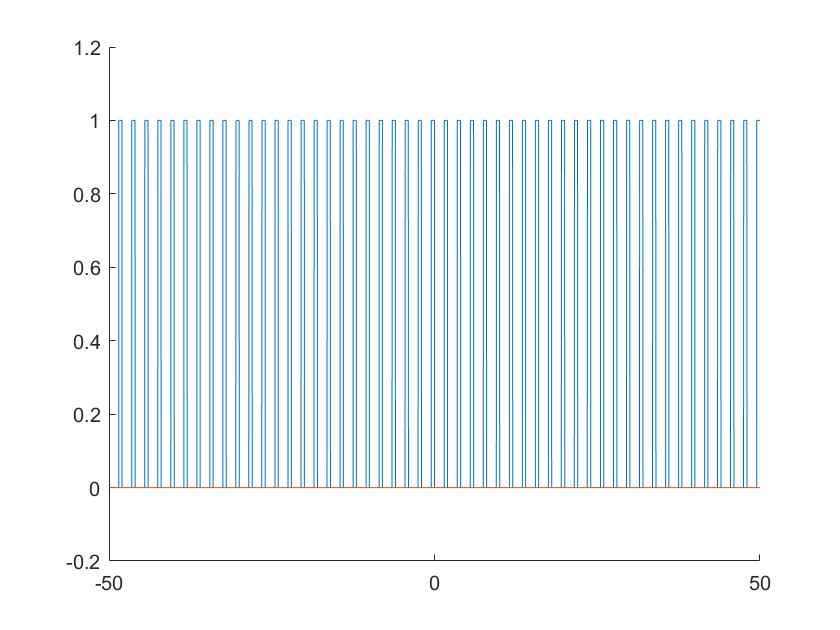
\includegraphics[scale=0.35]{fct6.jpg}
\caption{La fonction 6 après transformée de fourrier inverse}
\end{center} \end{figure}



\section{Transmission par modulation d'amplitude}
\textit(Calcul théorique)

\textit{Extraire s1 ou s2 : }\\
Pour extraire s1 ou s2 \textit{(figure~\ref{s1s2})}, il faut démoduler le signal c(t) \textit{(figure~\ref{c})} en le multipliant par $cos(2 \pi f t)$. On obtient alors le signal $d(t)$ \textit{(figure~\ref{d})} puis on applique un filtre passe-bas pour récupérer s1 ou s2 sur le signal ainsi obtenu \textit{(figure~\ref{s1demod})}.

\begin{figure}[h]
\begin{center}
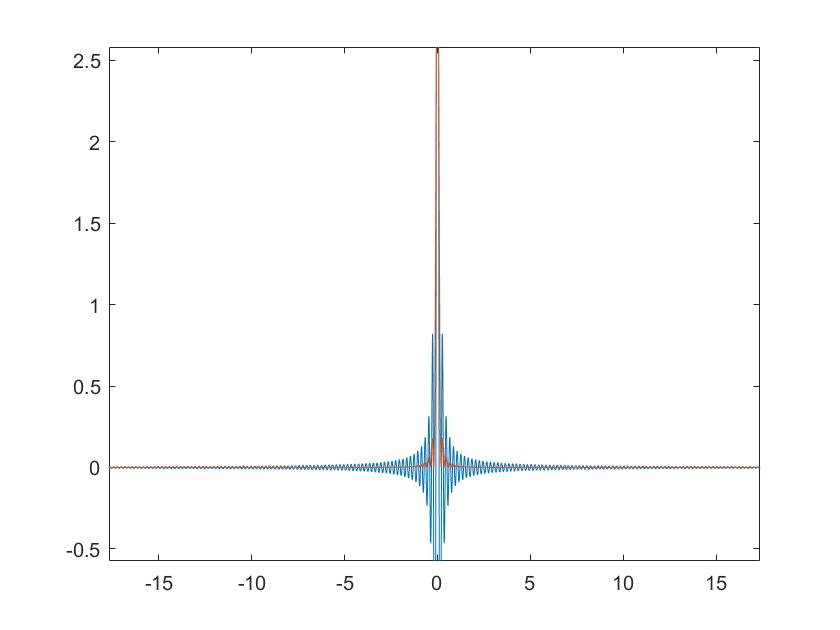
\includegraphics[scale=0.35]{tf_2signaux.jpg}
\caption{Les signaux $s1(t)$  en bleu et $s2(t)$ en orange}
\label{s1s2}
\end{center}
\end{figure}


\begin{figure}	\begin{center}
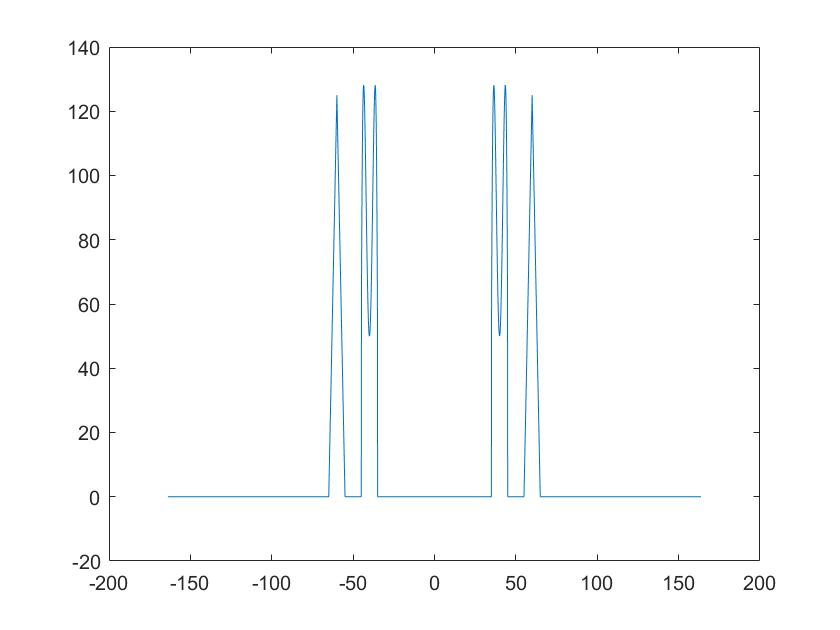
\includegraphics[scale=0.35]{tf_fctc.jpg}
\caption{Le signal $c(t)$. On peut remarquer que $f_1(t)$ = 40 Hz et $f_2(t)$ = 60Hz}
\label{c}
\end{center}	\end{figure}

\begin{figure}	\begin{center}
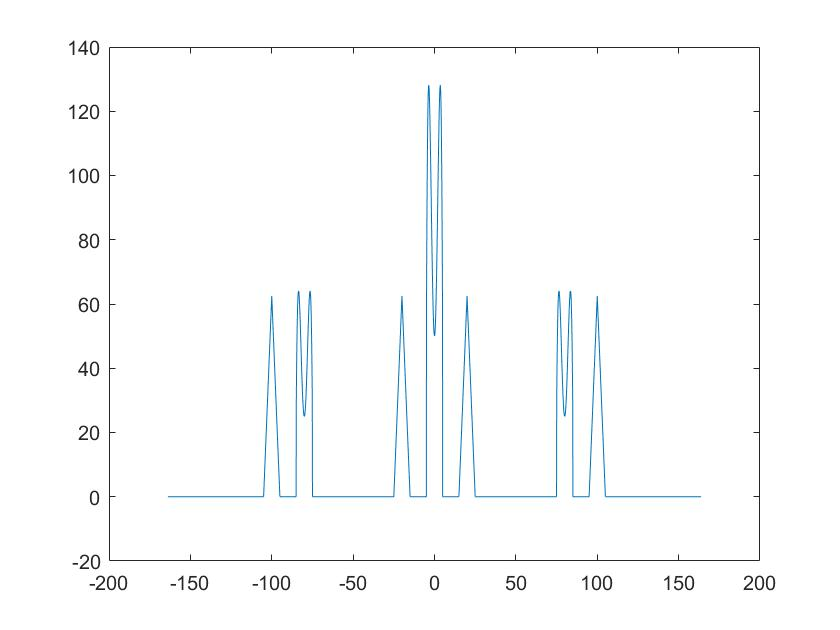
\includegraphics[scale=0.35]{Signal_d.jpg}
\caption{Le signal $d(t)$. On a démodulé le signal $c(t)$ avec $f_1(t)$}
\label{d}
\end{center}	\end{figure}

\begin{figure}	\begin{center}
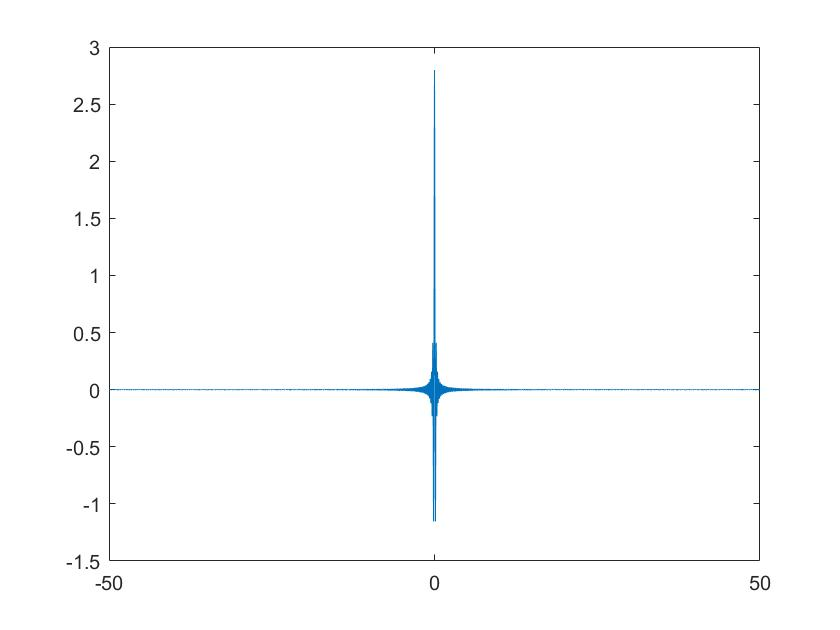
\includegraphics[scale=0.35]{s1_demodule.jpg}
\caption{Le signal $s1(t)$  obtenu après démodulation}
\label{s1demod}
\end{center}	\end{figure}



\textit{fréquence dépendante : }\\
Il faut faire attention à ne pas prendre des fréquences trop proches de celles de s1 ou s2.




\newpage

\section{Échantillonnage et aliasing	}

\section{Filtrage}

\section{Restauration d'image par filtre de Wiener}
Le but de cette partie est d'atténuer la dégradation (ici le flou) d'une image, par filtrage inverse. On va pour cela utiliser le filtre de Wiener : 
\[
	W(u,v) = \frac{1}{H(u,v)} * \frac{|H(u,v)|^2}{|H(u,v)|^2+\dfrac{P_b(u,v)}{P_i (u,v)}}	
\]

où $H(u,v)$ modélise la translation à l'origine du flou, et $P_i(u,v)$ ainsi que $P_b(u,v)$ sont deux spectres de puissance. $P_i(u,v)$ sera déterminé à partir d'une image de référence $i_r(x,y)$ et $P_B(u,v)$ est approximé par le spectre de puissance du bruit $b(x,y)$ qui apparaît lors du passage de $d_R(x,y)$ (l'image dégradée) à $d_Q(x,y)$ qui n'est codée que sur des nombres entiers.


\end{document}